\section{DIS pseudo-data generation}
\label{sec:dis_pseudodata}

Here we describe the procedure adopted in order 
to generate projections for the kinematic coverage
and experimental uncertainties associated to differential measurements
of neutrino-nucleus scattering at the LHC far-forward experiments.
%
First, we summarise the theoretical description of differential
neutrino scattering in terms of DIS structure functions and highlight
their PDF sensitivity.
%
Second, we present an  overview of the operative and proposed
LHC far-forward neutrino detectors that
will be considered in the present study and indicate their
key acceptance and performance parameters.
%
By convoluting the expected muon neutrino fluxes
with the acceptance and scattering rates of each
of these detectors,
we compute the foreseen event yields in bins of $x$, $Q^2$,
and $E_\nu$ and therefore the associated statistical uncertainties.
%
Finally, we estimate how the dominant systematic
uncertainties in each experiment translate into uncertainties in the predicted
event rates and use this information to complete the calculation of the experimental
covariance matrix.

\subsection{Neutrino DIS revisited}

The double-differential cross-section for neutrino-nucleus charged-current scattering,
see~\cite{Candido:2023utz} and references therein,
can be expressed in terms of 
independent structure functions $F_2^{\nu A}$, $xF_3^{\nu A}$
and $F_L^{\nu A}$:
\be
\label{eq:neutrino_DIS_xsec_FL}
\frac{d^2\sigma^{\nu A}(x,Q^2,y)}{dxdy} =  \frac{G_F^2s/4\pi}{\lp 1+Q^2/m_W^2\rp^2}\lc Y_+F^{\nu A}_2(x,Q^2) - y^2F^{\nu A}_L(x,Q^2) +Y_- xF^{\nu A}_3(x,Q^2)\rc  \, ,
\ee
where $Y_\pm = 1 \pm (1-y)^2$ and with a counterpart expression for anti-neutrino scattering,
\be
\label{eq:antineutrino_DIS_xsec_FL}
\frac{d^2\sigma^{\bar{\nu} A}(x,Q^2,y)}{dxdy} =  \frac{G_F^2s/4\pi}{\lp 1+Q^2/m_W^2\rp^2}\lc Y_+F^{\bar{\nu} A}_2(x,Q^2) - y^2F^{\bar{\nu} A}_L(x,Q^2) -Y_- xF^{\bar{\nu} A}_3(x,Q^2)\rc  \, ,
\ee
where $s=2m_N E_\nu$ being the neutrino-nucleon center of mass energy squared, $m_N$ is the nucleon mass,
$E_\nu$ is the incoming neutrino energy,
and the inelasticity is $y=Q^2/(2x m_n E_{\nu})$.
%
Structure functions depend only on $x$ and $Q^2$ while the differential
cross-section depends also on the neutrino energy $E_\nu$, or alternatively
on the inelasticity $y$.
%
Further, structure functions $F^{\nu A}_i(x,Q^2)$ and $F^{\bar{\nu} A}_i(x,Q^2)$ depend on the nuclear target $A$ entering
for the neutrino scattering through the nuclear modifications of the proton PDFs.

Eqns.~(\ref{eq:neutrino_DIS_xsec_FL}) and~(\ref{eq:antineutrino_DIS_xsec_FL}) are valid provided
the hadronic 
invariant mass $W$  is above the resonance threshold,
\be
W^2 = \lp m_N^2 + Q^2 \frac{(1-x)}{x} \rp \gsim \lp 2\,{\rm GeV} \rp^2\, ,
\ee
and in addition here we  restrict ourselves to the DIS region with perturbative momentum
transfers $Q^2$, such that
 structure functions are decomposed as
\be
\label{eq:sfs_pqcd}
 F^{\nu A}_i(x,Q^2) = \sum_{j=q,\bar{q},g}\int_x^1 \frac{dz}{z}\, C_{i,j}^{\nu N}(z,\alpha_s(Q^2))f^{(A)}_j\lp \frac{x}{z},Q^2\rp \, , \quad i = 2,3,L \, .
 \ee
%
in terms of a convolution of partonic scattering cross-sections  $C_{i,j}^{\nu N}(x,\alpha_s)$ and
of process-independent PDFs $f^{(A)}_j\lp x,Q^2\rp$.
%
A similar expression holds for charm production~\cite{Faura:2020oom}, which requires
accounting also for charm mass effects~\cite{Gao:2017kkx}.
 %
We discuss in Sect.~\ref{sec:settings} the theoretical
settings adopted~\cite{Candido:2022tld,yadism,Candido:2023utz,Carrazza:2020gss} to
evaluate predictions for
neutrino DIS structure functions, Eq.~(\ref{eq:sfs_pqcd}),
and for differential cross-sections,
Eqns.~(\ref{eq:neutrino_DIS_xsec_FL}) and~(\ref{eq:antineutrino_DIS_xsec_FL}),
in the kinematic range of relevance for LHC neutrinos.

 Each neutrino structure function provides complementary sensitivity
 to the partonic flavour decompositions of nucleons.
 %
 To illustrate this sensitivity, consider a leading order  calculation
 for a proton target with $n_f=4$ active quark flavours,
a diagonal CKM matrix and no heavy quark mass effects.
 %
 The resulting $F_2^{\nu p}$ and $xF_3^{\nu p}$ structure functions read
 \bea
 F_2^{\nu p}(x,Q^2) &=& 2x\lp f_{\bar{u}} + f_{d} + f_{s} + f_{\bar{c}} \rp(x,Q^2) \, , \nonumber  \\
 F_2^{\bar{\nu} p}(x,Q^2) &=& 2x\lp f_u + f_{\bar{d}} + f_{\bar{s}} + f_c \rp(x,Q^2) \, , \label{eq:neutrinoSFs_proton} \\
 xF_3^{\nu p}(x,Q^2) &=& 2x\lp -f_{\bar{u}} + f_d +f_s - f_{\bar{c}}\rp(x,Q^2)  \, , \nonumber\\
 xF_3^{\bar{\nu} p}(x,Q^2) &=& 2x\lp f_u - f_{\bar{d}} -f_{\bar{s}} + f_{c}\rp(x,Q^2) \, . \nonumber
 \eea
 The corresponding expressions for a neutron target are obtained from isospin symmetry
 \bea
 F_2^{\nu n}(x,Q^2) &=& 2x\lp f_{\bar{d}} + f_{u} + f_{s} + f_{\bar{c}} \rp(x,Q^2) \, , \nonumber  \\
 F_2^{\bar{\nu} n}(x,Q^2) &=& 2x\lp f_d + f_{\bar{u}} + f_{\bar{s}} + f_c \rp(x,Q^2) \, , \label{eq:antineutrinoSFs_neutron} \\
 xF_3^{\nu n}(x,Q^2) &=& 2x\lp -f_{\bar{d}} + f_u +f_s - f_{\bar{c}}\rp(x,Q^2)  \, , \nonumber\\
 xF_3^{\bar{\nu} n}(x,Q^2) &=& 2x\lp f_d - f_{\bar{u}} -f_{\bar{s}} + f_{c}\rp(x,Q^2) \, , \nonumber
 \eea
 while for an isoscalar, free-nucleon target denoted by $N$ one has
 \bea
 F_2^{\nu N}(x,Q^2) &=& 2x\lp f_{u^+} + f_{d^+} + 2f_s + 2f_{\bar{c}} \rp(x,Q^2) \, , \nonumber  \\
 F_2^{\bar{\nu} N}(x,Q^2) &=& 2x\lp f_{u^+} + f_{d^+} + 2f_{\bar{s}} + 2f_c \rp(x,Q^2) \, , \label{eq:neutrinoSFs_isoscalar} \\
 xF_3^{\nu N}(x,Q^2) &=& 2x\lp f_{u^-} + f_{d^-} +2f_s - 2f_{\bar{c}}\rp(x,Q^2)  \, , \nonumber\\
 xF_3^{\bar{\nu} N}(x,Q^2) &=& 2x\lp   f_{u^-} + f_{d^-}-2f_{\bar{s}} +2 f_{c}\rp(x,Q^2) \, , \nonumber
 \eea
 in terms of the valence and sea PDF combinations defined by
 \be
 f_{q^+} (x,Q^2)\equiv \lp f_{q}+f_{\bar{q}}\rp(x,Q^2) \, , \qquad
 f_{q^-} (x,Q^2)\equiv \lp f_{q}- f_{\bar{q}}\rp(x,Q^2) \, .
 \ee
 We note that even for isoscalar targets separate measurements
 for neutrinos and antineutrinos will not be equivalent, since in general neither $f_{s^-}$ nor
 $f_{c^-}$ are expected to vanish.

 In the projections presented in this work, when interpreting the LHC neutrino structure
 functions in terms of proton PDFs we will assume a isoscalar free-nucleon target and neglect
 nuclear PDF modifications, along the lines of Eq.~(\ref{eq:neutrinoSFs_isoscalar}).
 %
 On the other hand, when evaluating structure functions
 for a tungsten (W) target, we keep into account both
 nuclear corrections and that
 the target is not isoscalar when evaluating the physical observables.
 %
 We point out that accounting for nuclear target effects in a global proton
 PDF fit is straightforward by means of the procedure developed
 in~\cite{Ball:2020xqw,Ball:2018twp}.

 It is illustrative to compare the PDF dependence of neutrino structure functions
 at LO with that of their counterparts for neutral-current
 scattering with a charged lepton projectile.
 %
 Within the same assumptions, for energies below
 the $Z$-boson mass, $Q^2 \ll m_Z$, the corresponding
 partonic decomposition is
 the 
 \bea
 F_2^{\ell p}(x,Q^2) &=& x\lp \frac{4}{9}\lc f_{u^+} + f_{c^+}\rc
 + \frac{1}{9}\lc f_{d^+} + f_{s^+}\rc\rp(x,Q^2) \, , \nonumber  \\
 F_2^{\ell n}(x,Q^2) &=& x\lp \frac{4}{9}\lc f_{d^+} + f_{c^+}\rc
 + \frac{1}{9}\lc f_{u^+} + f_{s^+}\rc\rp(x,Q^2) \, ,\label{eq:NC_chargedlepton}   \\
 F_2^{\ell N}(x,Q^2) &=& x\lp \frac{5}{18}\lc f_{u^+} + f_{d^+}\rc
 + \frac{1}{9} f_{s^+} + \frac{4}{9} f_{c^+} \rp(x,Q^2) \, , \nonumber  
 \eea
 with $xF_3$ being negligible in this region.
 %
 Eq.~(\ref{eq:NC_chargedlepton}) showcases the complementarity between
 neutrino and charged-lepton DIS in terms of sensitivity
 to the flavour PDF decomposition.

 \subsection{Far-forward neutrino detectors at the LHC}
 \label{sec:neutrinoDetectors}

 As we discuss below, the calculation of differential neutrino scattering event rates
 at the LHC far-forward detectors requires two main ingredients: the energy
 and flavour dependence of the incoming neutrino flux crossing
 the detector fiducial volume, on the one hand,
 and the scattering rates within the same fiducial volume, on the other hand.
 %
 In this section, we summarise the main features of each of the ongoing and future
 far-forward detectors considered in this study, in particular concerning
 their acceptance, geometry, and neutrino detection method.
 %
 We also indicate the expected performance of the three FPF detectors
 and how this translates into the dominant experimental systematic
 uncertainties.
 %
 Since for the projection studies considered in this work we focus on muon
 neutrino scattering, we will focus the subsequent discussion on the detection
 performance of this neutrino flavour.

 Table~\ref{tab:FPF_experiments} indicates
 the rapidity coverage, target material,
 muon neutrino acceptance, and the identification and reconstruction performance
 for each of the far-forward LHC neutrino experiments considered
 in this work.
 %
 More details of the information listed in this table is provided
 in the following.

  %-----------------------------------------------------------------
\begin{table}[t]
  \centering
  \small
  \renewcommand{\arraystretch}{1.50}
\begin{tabularx}{\textwidth}{Xccccc}
\toprule
Detector &  Rapidity &  Target & Lepton sign & Acceptance  & Performance \\
\midrule
\multirow{2}{*}{FASER$\nu$}  &   &   Tungsten  & \multirow{2}{*}{muons}      &     &         \\
  &   &   (1.1 ton)  &       &     &         \\
\midrule
\multirow{2}{*}{SND@LHC}  & \multirow{2}{*}{ $7.2 \le \eta_\nu \le 8.4$}   &  Tungsten   &       &       &       \\
  &   &  (0.83 ton)   &       &       &       \\
\midrule
\midrule
\multirow{3}{*}{FASER$\nu$2}  &   & \multirow{2}{*}{Tungsten}    &   \multirow{3}{*}{only muons}     &   $E_\ell \gsim 100$ GeV  &    $\delta E_\ell \sim 30\% $     \\
  &   &  \multirow{2}{*}{(20 ton)}   &       &  $\tan \theta_\ell \lsim 0.5$   &   $\delta \theta_\ell \sim 1$ mrad      \\
  &   &     &       &  reconstructed $E_h$ \& charm ID   &  $\delta E_h \sim 30\%$        \\
\midrule
\multirow{3}{*}{AdvSND~(far)}  &   \multirow{3}{*}{ $7.2 \le \eta_\nu \le 8.4$}  &
\multirow{2}{*}{Tungsten}   &   \multirow{3}{*}{only muons}    &  $E_\mu \gsim 20 $ GeV  & \multirow{3}{*}{n/a}          \\
  &   &   \multirow{2}{*}{(5 ton)}  &        & $\theta_\mu \lsim 0.15, \theta_e \lsim 0.5$     &           \\
  &   &     &       &  reconstructed $E_h$   &           \\
\midrule
\multirow{3}{*}{FLArE}  & \multirow{3}{*}{Liquid Argon}  &  & \multirow{3}{*}{ maybe muons}  &  $E_\mu \lsim 2$ GeV, $E_e \lsim 1$ TeV    &    $\delta E_e \sim 5\% $ \\
&   &     &   & $\theta_\mu \lsim 0.4$, $\theta_e \lsim 0.5$ &    $\delta \theta_e \sim 15 $ mrad   \\
 &   &     &  & reconstructed $E_h$  &    $\delta E_h \sim 30\% $   \\
  \bottomrule
\end{tabularx}
\vspace{0.2cm}
\caption{\small For each of the far-forward LHC neutrino experiments considered
  in this work, we indicate their rapidity coverage, target material, whether
  they can identify the sign of the outgoing charged lepton,
  the detector acceptance for the charged lepton and hadronic final state,
  and the expected reconstruction performance.
  %
  We consider separately the acceptance and performance for electron and muon
  neutrinos.
  %
  Tau neutrinos have much lower production rates and are not considered in this study.
  %
  See the description of each experiment in the text for more details.
  \label{tab:FPF_experiments}
}
\end{table}
%-----------------------------------------------------------------

\paragraph{FASER$\nu$.}
%
The ForwArd Search ExpeRiment (FASER) detector and its companion FASER$\nu$
are located at the TI12 tunnel of the CERN accelerator complex.
%
Both detectors are aligned
with the collision axis LOS  and have been taking data since the begin of Run III.
%
Neutrino scattering takes place in the FASER$\nu$
detector, composed by interleaved emulsion and tungsten plates and
adding up to a mass of 1.1 tons with a fiducial volume of $20~\rm{cm} \times 25~\rm{cm} \times 30~{\rm cm}$.
%
The FASER/FASER$\nu$ apparatus is immersed in a magnetic field which enables charged lepton
identification, provided by two 1 m-long dipole magnets with $B=0.57$ T
and another 1.5 m-long magnet in front of the spectrometer. 
%
Neutrino detection and identification can be carried out either using the emulsion
films of FASER$\nu$2, which have the key benefit of excellent position and angular resolution,
or instead using the electronic detector components of FASER, which enable the tagging
of the outgoing downstream energetic muons. 

\paragraph{SND@LHC.}
%
In the same manner as FASER, the SND@LHC experiment is located in a service tunnel (TI18)
around 500 meters from the ATLAS interaction point and has been taking data
since the  beginning of Run 3.
%
SND@LHC is installed off the LOS axis in order to cover the neutrino
pseudo-rapidity range of $7.2 \le \eta_\nu \le 8.4$.
%
With a total fiducial volume of 830 kg, it is composed by tungsten plates,
where neutrino scattering takes place, interleaved with nuclear emulsions and electronic tracker
components.
%
Downstream, the scattering volume is followed by a hadronic calorimeter and a muon tracking system.
%
The electromagnetic
 and hadronic energy deposits can be measured at the electronic detectors, with the emulsion
 components providing vertex reconstruction.
 %
 The lack of magnetic field prevents the charge-sign identification of the outgoing charged leptons.

\paragraph{FASER$\nu$2.}
%
A 20-ton neutrino experiment located on the line of sight (LOS)
of the LHC neutrino beam.
%
It is based on an emulsion-based detector optimised to identify heavy flavor particles, including
tau leptons and charm and beauty particles, arising from neutrino interactions.
%
The FASER$\nu$2 detector is composed of 3300 emulsion layers interleaved with 2-mm-thick tungsten plates,
for a total volume of  tungsten of $40~\rm{cm} \times 40~\rm{cm} \times 6.6~{\rm m}$.
%
The combination of FASER$\nu$2  with the nearby FASER2 detector, equipped with a spectrometer, makes measurements of the outgoing muon charge possible.

 \paragraph{AdvSND.}
 %
 This experiment consists on  two detectors, a far-detector to be installed
 at the FPF with a coverage in neutrino pseudorapidity $\eta_\nu$ of $7.2 \le \eta_\nu \le 8.4$
 (hence off-LOS) and a near detector installed somewhere else in LHC
 complex and covering the range $4 \le \eta_\nu \le 5$.
 %
 In the following we focus on the AdvSND far-detector.
 %
 It would be
 composed (from upstream to downstream) by a target region
 for  vertex reconstruction and electromagnetic energy measurement, followed  by a hadronic calorimeter, a  muon identification system, and finally  a magnet enabling muon charge and momentum measurements.
 %
 The target region of the detector, where the neutrino interactions take place, is made of thin sensitive layers interleaved with tungsten plates, for a total mass of 5 tons.
 %
 This detector configuration will be able to track muons with energy $E_\nu \gsim 20$ GeV
 within an acceptance of 100 mrad and provide information on the charge
 of the  outgoing muon thanks to its magnet.
 %
 The total energy of the hadronic final state will be measured
 in the hadronic calorimeter.

 \paragraph{FLArE.}
 %
 Building upon recent progress in liquid noble gas neutrino detectors over the last decade (ICARUS, MicroBooNE, SBND, ProtoDUNE, DUNE), this experiment relies on a modularized liquid argon (LAr) time projection detector.
 %
 The use of LAr as target is particularly beneficial for final-state particle identification, track angle, and kinetic energy measurements with sub-millimeter spatial resolution in all three dimensions.
 %
 FLArE is suitable to identify high-energy neutrinos ($E_\nu \gsim 100$ GeV)  from all three generations
 while  fully containing the events as required for kinematic reconstruction.
 %
 The detector will be equipped with a magnetized hadron/muon calorimeter downstream of the liquid argon volume
 for muon charge and momentum measurements.
 %
 With an expected fiducial (active) mass of 10 tons (30 tons), FLArE will
 detect muon neutrinos with energies  $E_\mu\lsim 1.5~\rm{TeV}$ and
 scattering angles up to 0.4 mrad.
 %
 Reconstruction of the total energy of the hadronic final state will also
 possible. 
 %
 In terms of performance, the targets
 are $\delta E_\mu \sim$30\% of muon energy resolution and
 $\delta \theta_\mu \sim 5$ mrad of muon angular  resolution.

\subsection{Differential event rate calculation}
\label{sec:pseudo-data_generation}

For each of the LHC far-forward neutrino detectors
described in Table~\ref{tab:FPF_experiments}, we generate
projections for the expected precision of DIS structure function
measurements as follows.
%
The goal is to quantify the number of reconstructed charged-current neutrino interaction
events taking place in the fiducial volume of the detector in bins of Bjorken-$x$,
momentum transfer $Q^2$, and neutrino energy $E_\nu$, that is,
\be
\label{eq:event_yields}
N_{\rm ev}^{(i)}\lp \nu_e ; E_{{\rm min}}^{(i)} \le E_\nu \le E_{{\rm max}}^{(i)} ,\,
x_{{\rm min}}^{(i)} \le x \le x_{{\rm max}}^{(i)} ;\, Q_{{\rm min}}^{2(i)} \le Q^2 \le Q_{{\rm max}}^{2(i)}\rp
\, ,\quad i=1,\ldots, N_{\rm bins} \, ,
\ee
for electron neutrinos and for each of the bins composing the measurement, and with similar
expressions applying for muon and tau neutrinos and antineutrinos.
%
These event yields determine the statistical
precision associated to a measurement of the double-differential cross-sections
Eqns.~(\ref{eq:neutrino_DIS_xsec_FL}) and~(\ref{eq:antineutrino_DIS_xsec_FL}).
%
Subsequently, we account for the expected reconstruction performance of the detector
in order to estimate the systematic uncertainties associated to these event yields.
%
The choice of the binning is in principle arbitrary, and here we define them
to ensure that Gaussian statistics hold for all the bins of the measurement.

In this calculation we assume the neutrino fluxes provided by the calculation
of~\cite{Kling:2021gos} and neglect the associated uncertainties.
%
The bin-by-bin integrated event yields in Eq.~(\ref{eq:event_yields}) are
obtained by convoluting the incoming neutrino fluxes, for a given geometric acceptance
of the target detector, with the corresponding neutrino differential cross-sections
Eqns.~(\ref{eq:neutrino_DIS_xsec_FL}) and~(\ref{eq:antineutrino_DIS_xsec_FL}).
%
As we further discuss in Sect.~\ref{sec:settings}, theoretical predictions
for the latter are computed with {\sc\small YADISM} interfaced to {\sc\small PineAPPL}
to produce fast precomputed interpolation grids.
%
Differential event yields are therefore evaluated using
\begin{equation}
  \label{eq:event_yields}
   N_{\rm ev}^{(i)} = n_T L_T\int_{Q^{2(i)}_{\rm min}}^{Q^{2(i)}_{\rm max}}\int_{x^{(i)}_{\rm min}}^{x^{(i)}_{\rm max}}\int_{E_{\rm min}^{(i)}}^{E_{\rm max}^{(i)}} \frac{dN_{\nu}(E_\nu)}{dE_{\nu}}\left(\frac{d^2\sigma(x,Q^2,E_{\nu})}{dxdQ^2}\right) dQ^2 dx dE_{\nu} \, ,\quad i=1,\ldots, N_{\rm bins} \, ,
\end{equation}
with $n_T$ is the nuclear density of the target detector material and $L_T$ its length.
%
The incoming neutrino fluxes, which include the geometric acceptance of the considered detector,
are encoded in $dN_{\nu}(E_\nu)/dE_{\nu}$.
%
We consider the scattering of muon neutrinos, characterised by the highest rates, and in some cases
we present results also for electron neutrinos.
%
We have verified that the differential event yield calculation
implemented in Eq.~(\ref{eq:event_yields}), when extrapolated to a single bin
covering the full detector acceptance,
is consistent with the fiducial interaction rates presented in~\cite{Feng:2022inv}.
%
The triple integral in  Eq.~(\ref{eq:event_yields}) is evaluated numerically by means
of Monte Carlo sampling, by generating sampling $N_{\rm mc}$ points in the $\lp x,Q^2,E_{\nu}\rp$ space
with the constraint that $0 < y = Q^2/2m_N E_{\nu }x <1 $
and then  integrating over the bin range:
\begin{equation}
    N_{\rm ev}^{(i)} \approx n_T L_T \frac{(Q^{2(i)}_{\rm max}-Q^{2(i)}_{\rm min})(x^{(i)}_{\rm max}-x^{(i)}_{\rm min})(E_{\rm max}^{(i)}-E_{\rm min}^{(i)})}{N_{\rm mc}}\times \sum_{j=1}^{N_{\rm mc}} \frac{dN_{\nu}(E^{(j)}_\nu)}{dE_{\nu}}\left(\frac{d^2\sigma(x^{(j)},Q^{2(j)},E^{(j)}_{\nu})}{dxdQ^2}\right) \, ,
    \label{MCintegration}
\end{equation}
and where $N_{\rm mc}$ is chosen to be large enough such that residual Monte Carlo integration
uncertainties are negligible.


where $f(x_i,Q^2_i,E_{\nu ,i}) = \frac{dN_{\nu}}{dE_{\nu,i}}\left(\frac{d^2\sigma(x_i,Q^2_i,E_{\nu,i})}{dxdQ^2}\right)$. 

The statistical uncertainty for each bin is then defined by a Gaussian distribution with fractional uncertainty $1/\sqrt{N{\rm ev}/{\rm bin}}$, i.e. $\delta N_{\rm ev}/{\rm bin} = \sqrt{N_{\rm ev}} /{\rm bin}$


  Following this prescription, we can produce plots which characterize the event rate for a particular neutrino species at a particular experiment. 

Results for FASER$\nu$2 can be found \href{https://github.com/juanrojochacon/FPF-WG1/tree/main/results}{here}. The .txt files will display which neutrino species was considered, and also compile experimental geometries and target details in the header. In the sub-folder \href{https://github.com/juanrojochacon/FPF-WG1/tree/main/results/Summaries}{summaries}, plots can be found which show the event rate in $x,Q^2$ space, integrating over the entire neutrino spectrum. The event rate for muon neutrinos at FASER$\nu$2 is shown in Fig~\ref{fig:fasernu2_muon}.

\begin{figure}[h]
    \centering
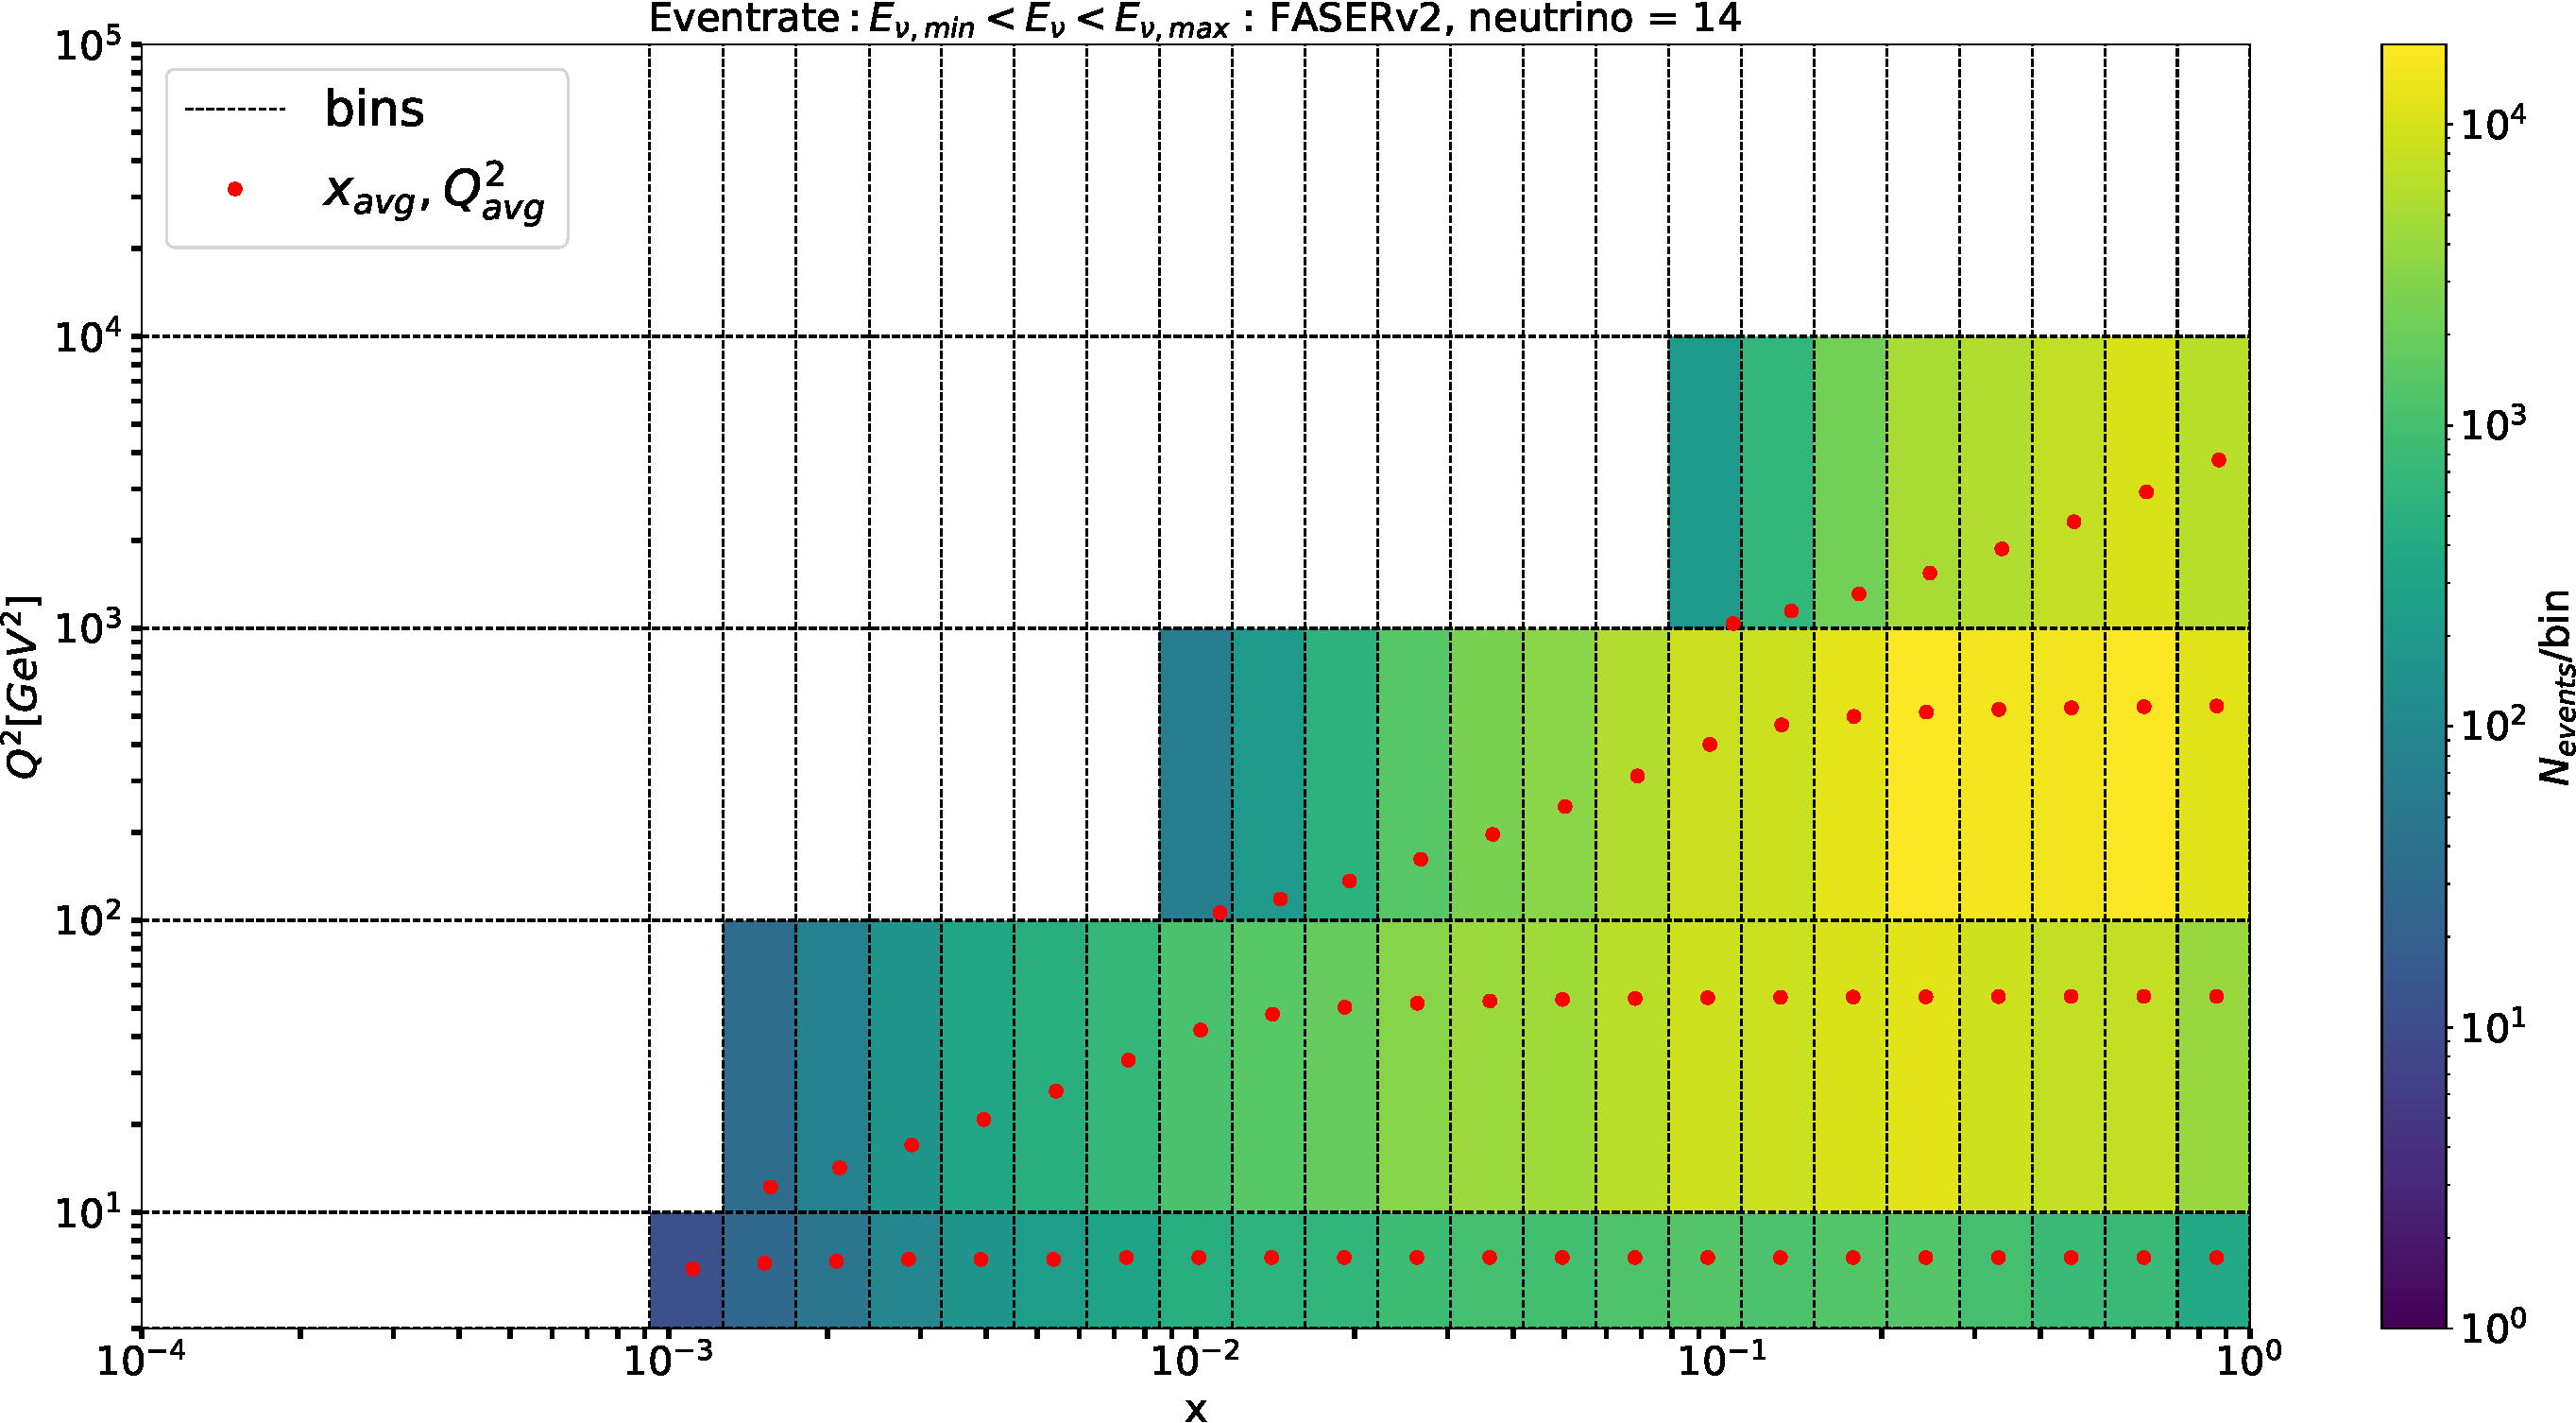
\includegraphics[width=1\textwidth]{plots/Nevent_FASERv2_14.pdf}
    \caption{Event rate per bin for muon neutrinos at FASER$\nu$2. Bins are denoted by dashed grid, and the red dot indicates the weighted average of $x,Q^2$ points in each bin. The total number of muon neutrino events calculated is $\approx2.6\times 10^5$. Note that bins were chosen somewhat arbitrarily, and can be iterated to improve PDF fits }
    \label{fig:fasernu2_muon}
\end{figure}

\subsection{Estimating systematic uncertainties}

We now wish to understand the impact of systematic uncertainties on the event rate in $(x,Q^2,E_{\nu})$ space. For each experiment, the observables $E_{l},E_{h},\theta$ are related to $(x,Q^2,E_{\nu})$ by 

\begin{align}
E_{\nu} = E_l + E_h \nonumber \\
Q^2 = 4E_lE_{\nu}\sin^2{\theta/2} \nonumber \\
x = \frac{Q^2}{2m_N(E_{\nu} - E_l)}.
\end{align}

We wish to sample over the space of observables, $(E_{l},E_{h},\theta)$, perform  cuts based on detector performance, calculate the event rates, and then smear this sampling according to experimental uncertainties to estimate the uncertainty on the event rate. 

Taking FASER${\nu}$2 as an example, we can write the experimental cuts and uncertainties as 

\begin{align}
100 < E_l < E_{\nu,{\rm max}} , \delta E_l = 30\% \nonumber \\
100 < E_h < E_{\nu,{\rm max}} , \delta E_h = 50\% \nonumber \\
0 < \theta < \tan^{-1}(0.5) , \delta\theta = 1~{\rm mrad}
\label{fasernu2systematic_errors}
\end{align}

We first generate a MC dataset, $D_0$, over this space with $N = 10^7$ samples and calculate $x,Q^2,E_{\nu}$ for each event, removing samples with $y > 1$. We then integrate according to Eq. \ref{MCintegration} to produce a distribution of events with bins in $x,Q^2,E_{\nu}$. We then smear each sample according to a Gaussian distribution with widths given by Eq.~\ref{fasernu2systematic_errors} to produce a new data set $D_i$ and repeat to produce $M = 10$ event distributions($M>10$ can later be used, but $M = 10$ appears to be stable). For each bin we take the standard deviation to produce the systematic errors per bin (denoted as "N\textunderscore sys\textunderscore errs" in files named "binned\textunderscore sys-events... .txt" \href{https://github.com/juanrojochacon/FPF-WG1/tree/main/results}{here}). 

For FASER${\nu}$2, the systematic errors typically dominate over statistical errors, at about $10\%$. 

\begin{figure}[h]
    \centering
    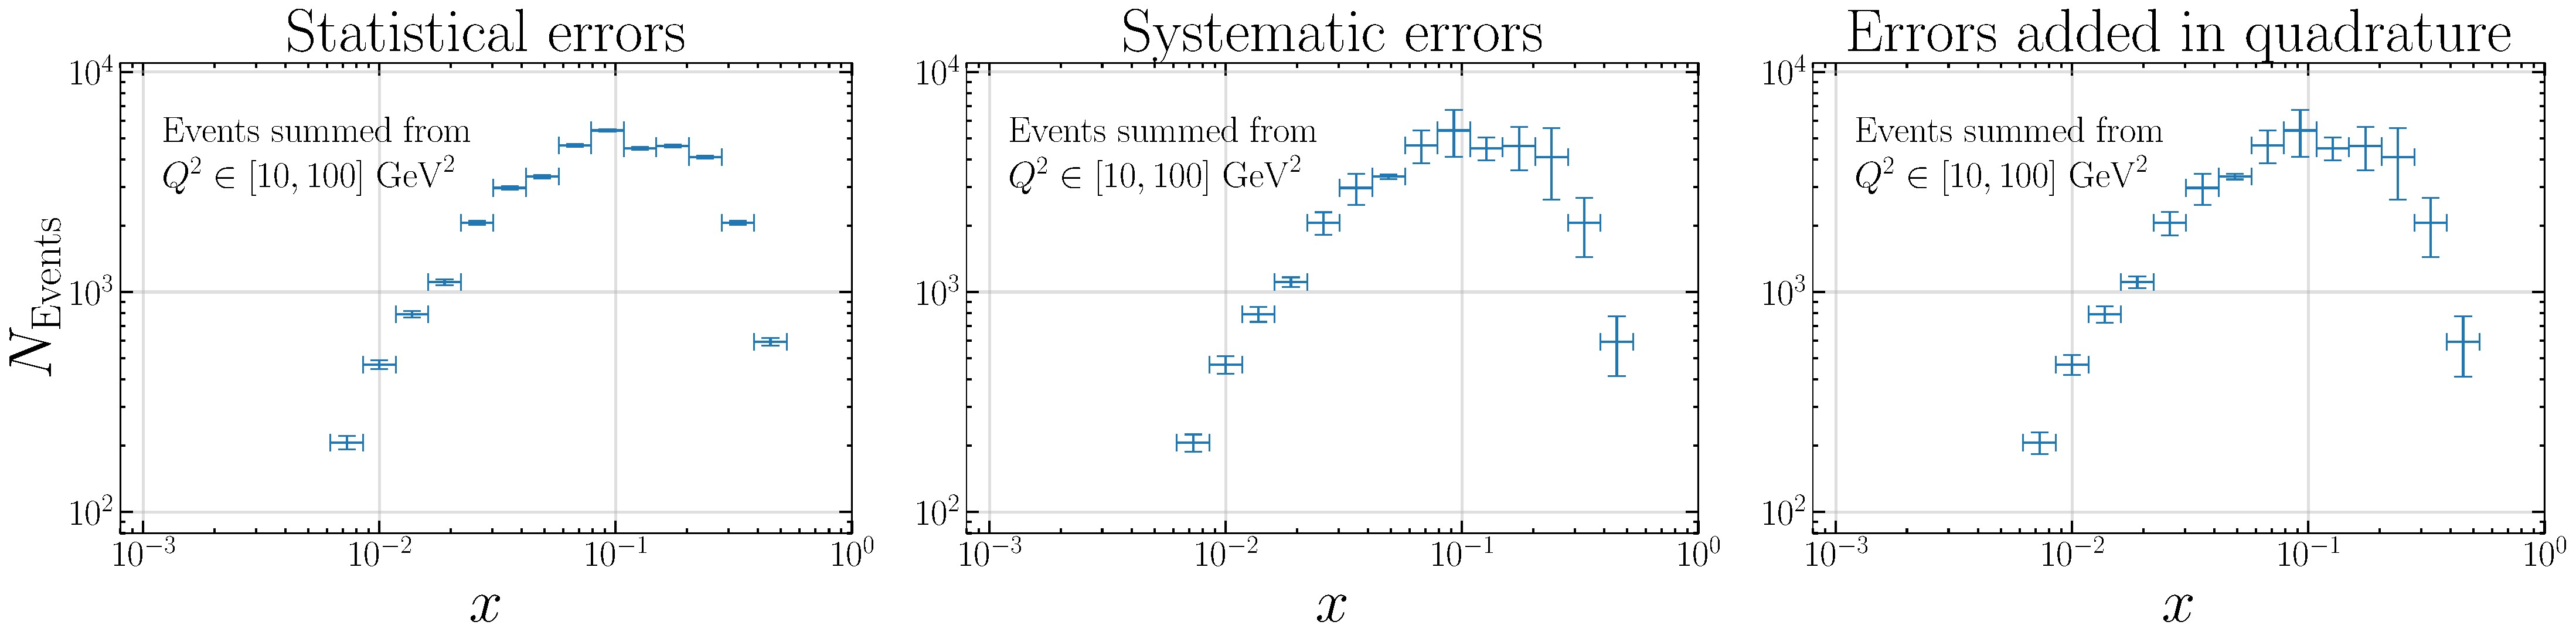
\includegraphics[width = 1\textwidth]{plots/error_plot_FASERv2_14.pdf}
    \caption{Event rates with error bars at FASER$\nu$2 for $\nu_{\mu} N \rightarrow \mu^- X$} summed over $Q^2$. The error bars along the x-axis showing the width of the $x$-bins, and are not showing any type of error.
    \label{fig:my_label}
\end{figure}

